\documentclass{article}

% if you need to pass options to natbib, use, e.g.:
\PassOptionsToPackage{numbers, compress}{natbib}
% before loading neurips_2026

% The authors should use one of these tracks.
% Before accepting by the NeurIPS conference, select one of the options below.
% 0. "default" for submission
\usepackage[main,final]{neurips_2026}
\usepackage[numbers]{natbib}
\makeatletter
\renewcommand{\@noticestring}{}
\makeatother

% the "default" option is equal to the "main" option, which is used for the Main Track with double-blind reviewing.
% 1. "main" option is used for the Main Track
%  \usepackage[main]{neurips_2026}
% 2. "position" option is used for the Position Paper Track
%  \usepackage[position]{neurips_2026}
% 3. "eandd" option is used for the Evaluations & Datasets Track
 % \usepackage[eandd]{neurips_2026}
% 4. "creativeai" option is used for the Creative AI Track
%  \usepackage[creativeai]{neurips_2026}
% 5. "sglblindworkshop" option is used for the Workshop with single-blind reviewing
 % \usepackage[sglblindworkshop]{neurips_2026}
% 6. "dblblindworkshop" option is used for the Workshop with double-blind reviewing
%  \usepackage[dblblindworkshop]{neurips_2026}
% 7. "education" option is used for the Education Track
%  \usepackage[education]{neurips_2026}


% After being accepted, the authors should add "final" behind the track to compile a camera-ready version.
% 1. Main Track
 % \usepackage[main, final]{neurips_2026}
% 2. Position Paper Track
%  \usepackage[position, final]{neurips_2026}
% 3. Evaluations & Datasets Track
 % \usepackage[eandd, final]{neurips_2026}
% 4. Creative AI Track
%  \usepackage[creativeai, final]{neurips_2026}
% 5. Workshop with single-blind reviewing
%  \usepackage[sglblindworkshop, final]{neurips_2026}
% 6. Workshop with double-blind reviewing
%  \usepackage[dblblindworkshop, final]{neurips_2026}
% Note. For the workshop paper template, both \title{} and \workshoptitle{} are required, with the former indicating the paper title shown in the title and the latter indicating the workshop title displayed in the footnote.
% For workshops (5., 6.), the authors should add the name of the workshop, "\workshoptitle" command is used to set the workshop title.
% \workshoptitle{WORKSHOP TITLE}
% 7. Education Track
% \usepackage[education, final]{neurips_2026}

% "preprint" option is used for arXiv or other preprint submissions
 % \usepackage[preprint]{neurips_2026}

% to avoid loading the natbib package, add option nonatbib:
%    \usepackage[nonatbib]{neurips_2026}

\usepackage[utf8]{inputenc} % allow utf-8 input
\usepackage[T1]{fontenc}    % use 8-bit T1 fonts
\usepackage{hyperref}       % hyperlinks
\usepackage{url}            % simple URL typesetting
\usepackage{booktabs}       % professional-quality tables
\usepackage{amsfonts}       % blackboard math symbols
\usepackage{nicefrac}       % compact symbols for 1/2, etc.
\usepackage{microtype}      % microtypography
\usepackage{xcolor}         % colors
\usepackage{amsmath}
\usepackage{float}

% \usepackage{tikz}
% \tikzset{
%   vmark/.style={circle, fill=black, inner sep=2pt},
%   umark/.style={circle, draw=black, inner sep=2pt},
%   bmark/.style={rectangle, fill=black, inner sep=2pt},
%   amark/.style={rectangle, draw=black, inner sep=2pt}
% }




\usepackage{tikz}
\usetikzlibrary{shapes.geometric}

\tikzset{
  vmark/.style={circle,draw=black,fill=black,inner sep=1.5pt},
  umark/.style={rectangle,draw=black,fill=black!45,inner sep=1.6pt},
  bmark/.style={diamond,draw=black,fill=white,inner sep=1.4pt},
  amark/.style={regular polygon,regular polygon sides=3,draw=black,fill=white,inner sep=1.1pt},
mmark/.style={star,star points=5,star point ratio=2.2,draw=black,fill=black!25,inner sep=0.9pt},
}




\newcommand{\djoint}{\Delta_{\text{Joint}}}
\newcommand{\daware}{\Delta_{\text{Aware}}}

% Note. For the workshop paper template, both \title{} and \workshoptitle{} are required, with the former indicating the paper title shown in the title and the latter indicating the workshop title displayed in the footnote. 
\title{Two New Text-Tabular Datasets for MulTaBench}


% The \author macro works with any number of authors. There are two commands
% used to separate the names and addresses of multiple authors: \And and \AND.
%
% Using \And between authors leaves it to LaTeX to determine where to break the
% lines. Using \AND forces a line break at that point. So, if LaTeX puts 3 of 4
% authors names on the first line, and the last on the second line, try using
% \AND instead of \And before the third author name.


\author{%
  Noa Bamberger\\
  Technion - Israel Institute of Technology \\
  NLP (00970215) - Track 2 (Benchmark Track) \\
  \texttt{noabamberger@campus.technion.ac.il} \\
}


\begin{document}


\maketitle


% \begin{abstract}
% MulTaBench is a dedicated benchmark for multimodal tabular learning with text and image modalities. Expanding it with qualifying datasets broadens domain diversity and supports more robust, generalizable evaluations of multimodal models. Using the official MulTaBench curation protocol, we curate and evaluate two new text-tabular datasets across five tabular learners (TabM, CatBoost, LightGBM, TabPFN~v2, and TabPFN-2.5) under four experimental conditions. Both datasets demonstrate substantial multimodal improvements over unimodal baselines. \emph{Vietnam housing} qualifies across all five learners, exhibiting strong joint signal and statistically significant target-aware representation (TAR) gains. \emph{Udemy courses} also satisfy the benchmark acceptance threshold on a majority of learners (3 of 5), though its TAR effect does not reach statistical significance when pooled across folds. Finally, we detail the automated mining pipeline used to screen candidates and discuss two common screening shortcuts that we assess to be invalid.
% \end{abstract}

% ***********TO D0: make sure that what I changed is ok**************
\begin{abstract}
MulTaBench is a dedicated benchmark for multimodal tabular learning with text and image modalities. Expanding it with qualifying datasets broadens domain diversity and supports more robust, generalizable evaluations of multimodal models. Using the official MulTaBench curation protocol, we screened 232 candidate datasets through an automated pipeline, fully evaluated five candidates across five tabular learners (TabM, CatBoost, LightGBM, TabPFN~v2, and TabPFN-2.5) under four experimental conditions, and identified two new text-tabular datasets that satisfied the acceptance criterion. Both datasets demonstrate substantial multimodal improvements over unimodal baselines. \emph{Vietnam housing} qualifies across all five learners, exhibiting strong joint signal and statistically significant target-aware representation (TAR) gains. \emph{Udemy courses} also satisfy the benchmark acceptance threshold on a majority of learners (3 of 5), though its TAR effect does not reach statistical significance when pooled across folds. Finally, we detail the automated mining pipeline used to screen candidates and discuss two common screening shortcuts that we assess to be invalid.
\end{abstract}


\section{Introduction}

Real tables are rarely purely numerical: a property listing carries an address, a course
listing a title and an instructor name - free text beside numeric and categorical columns.
\emph{Text-tabular learning} asks how to use both channels at once. The question is not
rhetorical in that gradient-boosted trees remain very strong on structured data
\cite{grinsztajn,shwartzziv}. Accordingly, a multimodal method only earns its complexity on tables where
the text carries signal the structured block lacks, and vice versa. This makes \emph{dataset curation} a substantive research task rather than a simple data collection exercise. A benchmark
built from tables whose text merely restates their columns will report that multimodal methods offer little to no value added. MulTaBench \cite{multabench}
makes the requirement measurable in that a table is worth benchmarking only if (i) the joint model
beats \emph{both} unimodal baselines, and (ii) a text encoder adapted to the prediction target
beats a frozen one. Failing (i) collapses the task into pure tabular or pure NLP. Failing (ii)
exercises text encoding but not the target-aware representation learning that models such as
TabSTAR \cite{tabstar} are built around. This raises the practical question of how to identify, from a large pool of candidate datasets, those tables that actually satisfy these requirements.

Our contributions are therefore threefold: 
(1)~\textbf{The identification of two new text-tabular datasets} that qualify under the MulTaBench curation protocol: Vietnamese residential real-estate listings~\cite{dataset_vietnam_housing} (accepted across 5 of 5 tabular learners) and online-course listings~\cite{dataset_udemy_courses} (accepted across 3 of 5), both demonstrating consistent multimodal gains over unimodal baselines [Section~\ref{sec:results}].
(2)~\textbf{ The description of an end-to-end automated mining pipeline} for discovery, column typing, and leakage screening [section~\ref{sec:method}]. From an initial pool of 232 screened candidates, resource constraints limited full-grid evaluation to a small subset, from which these two datasets were validated [section~\ref{sec:results}]. We report the survival rates across each filtering stage to guide future data collection efforts [section~\ref{sec:method}].

\vfill

\noindent
\begin{minipage}{\linewidth}
\rule{0.45\linewidth}{0.4pt}

\vspace{2pt}

{\footnotesize
\url{https://github.com/noabamberger/NLP_MULTABENCH}
}
\end{minipage}

\newpage

(3)~\textbf{The explication of methodological insights into multimodal tabular curation}, demonstrating why common heuristic shortcuts - specifically, filtering structured columns by name and attempting to screen target awareness on reduced epochs or single folds - are unreliable and lead to invalid curation verdicts [section~\ref{sec:results}].






\section{Related Work}

\paragraph{Tabular learning.} Gradient-boosted decision trees - XGBoost \cite{xgboost},
LightGBM \cite{lightgbm} and CatBoost \cite{catboost} - are the default for tabular
prediction and remain competitive against deep architectures \cite{grinsztajn,shwartzziv}. Deep
tabular models have closed much of the gap: FT-Transformer \cite{fttransformer} adapted
attention to heterogeneous columns, and TabM \cite{tabm} reaches GBDT-level accuracy through
parameter-efficient ensembling of an MLP backbone. We use LightGBM, CatBoost and TabM.

\paragraph{Tabular foundation models.} TabPFN v2 \cite{tabpfnv2} performs in-context learning
over a synthetic prior, strong on small tables without per-dataset gradient training;
TabPFN-2.5 \cite{tabpfn25} extends it to larger inputs. Pretrained rather than fitted,
they respond differently to input representation changes than do trees.

\paragraph{Text and tables together.} One line of work serialises rows into sentences for a
language model (TabLLM \cite{tabllm}); another embeds string entries as entities to transfer
across tables (CARTE \cite{carte}). The line we follow keeps the tabular learner and encodes
text columns into features with a contrastive sentence encoder, E5 \cite{e5}, optionally
adapted to the target. TabSTAR \cite{tabstar} makes that adaptation central -
\emph{semantically target-aware} representations - and MulTaBench operationalises it as the
\texttt{ft} condition: an E5 encoder LoRA-tuned \cite{lora} on the target.

\paragraph{Benchmarks and curation.} MulTaBench \cite{multabench} is, to our knowledge, the
first multimodal-tabular benchmark to publish an executable acceptance rule for its own
datasets rather than a curated list alone. We reuse its reference implementation of that rule
verbatim (Section~\ref{sec:method}), so our verdicts and the benchmark's are one computation.

\section{Method: the criterion, the pipeline, and the datasets}
\label{sec:method}


\paragraph{The criterion.} Each dataset is evaluated with five learners - TabM, CatBoost,
LightGBM, TabPFN v2 and TabPFN-2.5 - under four conditions: \textbf{Unimodal Structured}
(tabular columns only), \textbf{Unimodal Unstructured} (text only), \textbf{Joint Frozen} (all
features, frozen E5-small-v2 embeddings) and \textbf{Joint Target-Aware} (TAR; all features,
E5 LoRA-tuned on the target). Text columns are embedded per column and compressed to 30
principal components; scores are $R^2$, as both our datasets are regression tasks. Writing
$\mu_c$ for the mean score over folds $0$-$4$ in condition $c$, rounded to three decimals
before differencing, a learner passes when
\begin{align}
\Delta_{\text{Joint}}
&= \mu_{\text{frozen}} - \max(\mu_{\text{struct}}, \mu_{\text{text}}) > \delta,
&
\Delta_{\text{Aware}}
&= \mu_{\text{TAR}} - \mu_{\text{frozen}} > \delta,
\end{align}
with $\delta = 0.001$; a dataset is accepted when at least 3 of the 5 learners pass
\emph{both}, a learner clearing only one contributing nothing. Every verdict here is computed
by the MulTaBench reference implementation of this rule, which asserts grid completeness
(5 folds $\times$ 4 conditions per learner) rather than averaging over gaps; we did not
reimplement the arithmetic.
To assess whether improvements over unimodal baselines ($\djoint$) and frozen representations ($\daware$) are consistent across evaluations, we also compute one-sample $t$-statistics testing $H_0: \Delta_{\text{Aware/Joint}} \le 0$ pooled over all 25 (learner, fold) evaluations.

\paragraph{Setup and fidelity.} All grids ran on Kaggle \cite{kaggle} T4 GPUs, the four conditions for a
learner always measured in one session so that no environment difference can enter a delta.
To ensure fidelity, we validated our setup against the benchmark's published artifacts in two steps. First, applying the curation acceptance rule to MulTaBench's released raw scores reproduced its $56 \times 10$ pass matrix with zero mismatched cells. Second, re-evaluating a representative reference dataset (\emph{Product Sentiment}) from scratch exactly matched published scores in the encoder-free baseline, while $\Delta_{\text{Joint}}$ agreed within $0.012$ with all signs matching (Appendix~\ref{app:anchor}).
% \begin{table}[t]
% \centering
% \small
% \caption{Mining-funnel yield; percentages are of the 232 discovered candidates. The stage-6
% screen used the flawed column filter of Appendix~\ref{app:validity}, so 16 is an upper bound.}
% \label{tab:funnel}
% \begin{tabular}{lrr}
% \toprule
% Stage & Count & Survival \\
% \midrule
% Discovered by search & 232 & --- \\
% Parsed successfully & 229 & 99\% \\
% Viable under typing/target gates & 120 & 52\% \\
% After removing false text columns (dates, identifiers) & 58 & 25\% \\
% After excluding domains already in MulTaBench & 34 & 15\% \\
% Passing a screen & 16 & 7\% \\
% Full grid attempted & 4 & --- \\
% \textbf{Survived scrutiny} & \textbf{2} & \textbf{$<1\%$} \\
% \bottomrule
% \end{tabular}
% \end{table}







\begin{table}[t]
\centering
\small
\caption{Mining-funnel yield.} 
\label{tab:funnel}
\begin{tabular}{lrr}
\toprule
Stage & Count & Survival \\
\midrule
Discovered by search & 232 & --- \\
Parsed successfully & 229 & 99\% \\
Viable under typing/target gates & 120 & 52\% \\
After removing false text columns (dates, identifiers) & 58 & 25\% \\
After excluding domains already in MulTaBench & 34 & 15\% \\
Passing a screen & 16 & 7\% \\
Full grid attempted & 5 & --- \\
\textbf{Survived scrutiny} & \textbf{2} & \textbf{$<1\%$} \\
\bottomrule
\end{tabular}
\end{table}



\paragraph{Mining pipeline.} 
Candidates were discovered through a programmatic search over public dataset repositories, then profiled, screened, and gridded (Table~\ref{tab:funnel}). Under our compute budget, the end-to-end yield of our current screening configuration was under $1\%$. Rather than brute-forcing hundreds of full grids, the pipeline focuses on maximizing candidate qualification before committing resources to complete evaluation.
For each candidate, the pipeline selects a target and partitions columns without
human annotation. Targets are rejected when they are identifiers or serial numbers, when one
value holds more than $20\%$ of the mass (a sentinel masquerading as a number), when
$|z|_{\max} > 5$, or when derived from the text from which they would be predicted. Columns
correlating with the target at Spearman $\rho \ge 0.95$ are dropped as leakage (Spearman, so
monotone-but-nonlinear leaks such as a rank column are caught). Column typing is inferred, not
declared, such that a non-numeric column counts as text at $\ge 100$ distinct values or $\ge 80\%$
uniqueness - and it fails mainly by promoting dates and identifiers into the text block,
which is what reduces 120 nominally viable candidates to 58. Two cost-saving shortcuts that
look obvious are measurably invalid (Appendix~\ref{app:validity}), so every positive $\djoint$
below was re-measured with the maximal structured block and every $\daware$ at $\ge 10$ epochs
over all five folds.

\paragraph{The two datasets.} Both specifications were derived using our automated pipeline:
\begin{itemize}
    \item \textbf{Vietnam housing} (\textsc{reg\_text\_houses\_vietnam\_2024}; 30{,}229 listings)~\cite{dataset_vietnam_housing}: Predicts \texttt{Price} (687 distinct values, $|z|_{\max} = 2.54$). Features include one free-form text column (\texttt{Address}) paired with six numeric and four categorical physical attributes (e.g., area, floors, bedrooms), none of which duplicate the address.
    \item \textbf{Udemy courses} (\textsc{reg\_text\_edu\_udemy\_academy}; 2{,}999 listings)~\cite{dataset_udemy_courses}: Predicts course price (28 distinct values, $|z|_{\max} = 3.00$). Features include two text columns (\texttt{course\_name}, \texttt{course\_instr}) paired with six numeric course statistics.
\end{itemize}



\section{Results}
\label{sec:results}

% \begin{table}[t]
% \centering
% \caption{Per-learner results on Kaggle T4; means over folds 0--4 rounded to three decimals
% before differencing, $\delta = 0.001$. Struct./Text/Frozen/TAR are the four conditions of
% Section~\ref{sec:method}. Both grids are complete: 100 cells, no gaps.}
% \label{tab:results}
% \small
% \begin{tabular}{llrrrrrrl}
% \toprule
% Dataset & Learner & Struct. & Text & Frozen & TAR & $\djoint$ & $\daware$ & Verdict \\
% \midrule
% Vietnam & CatBoost   & 0.341 & 0.322 & 0.632 & 0.636 & $+0.291$ & $+0.004$ & pass \\
% housing & LightGBM   & 0.342 & 0.310 & 0.592 & 0.607 & $+0.250$ & $+0.015$ & pass \\
%         & TabM       & 0.312 & 0.336 & 0.633 & 0.638 & $+0.297$ & $+0.005$ & pass \\
%         & TabPFN v2  & 0.342 & 0.340 & 0.646 & 0.647 & $+0.304$ & $+0.001$ & pass$^{\dagger}$ \\
%         & TabPFN-2.5 & 0.356 & 0.346 & 0.680 & 0.685 & $+0.324$ & $+0.005$ & pass \\
% \midrule
% Udemy   & CatBoost   & 0.297 & 0.210 & 0.480 & 0.501 & $+0.183$ & $+0.021$ & pass \\
% courses & LightGBM   & 0.261 & 0.212 & 0.479 & 0.474 & $+0.218$ & $-0.005$ & fail \\
%         & TabM       & 0.298 & 0.221 & 0.504 & 0.492 & $+0.206$ & $-0.012$ & fail \\
%         & TabPFN v2  & 0.299 & 0.162 & 0.435 & 0.437 & $+0.136$ & $+0.002$ & pass \\
%         & TabPFN-2.5 & 0.311 & 0.211 & 0.452 & 0.464 & $+0.141$ & $+0.012$ & pass \\
% \bottomrule
% \end{tabular}
% \vspace{2pt}
% \parbox{0.95\textwidth}{\footnotesize $^{\dagger}$ Knife-edge: the difference of rounded means
% is exactly $\delta$, clearing a strict $>$ only through float64 representation. Excluding it
% leaves 4 of 5, still accepted.}
% \end{table}





% \begin{table}[t]
% \centering
% \small

% \caption{Per-learner results on Kaggle T4.}
% \label{tab:results}




% \begin{tabular}{llrrrrrrl}
% \toprule
% Dataset & Learner & Struct. & Text & Frozen & TAR & $\djoint$ & $\daware$ & Verdict \\
% \midrule
% Vietnam & CatBoost   & 0.341 & 0.322 & 0.632 & 0.636 & $+0.291$ & $+0.004$ & pass \\
% housing & LightGBM   & 0.342 & 0.310 & 0.592 & 0.607 & $+0.250$ & $+0.015$ & pass \\
%         & TabM       & 0.312 & 0.336 & 0.633 & 0.638 & $+0.297$ & $+0.005$ & pass \\
%         & TabPFN v2  & 0.342 & 0.340 & 0.646 & 0.647 & $+0.304$ & $+0.001$ & pass$^{\dagger}$ \\
%         & TabPFN-2.5 & 0.356 & 0.346 & 0.680 & 0.685 & $+0.324$ & $+0.005$ & pass \\
% \midrule
% Udemy   & CatBoost   & 0.297 & 0.210 & 0.480 & 0.501 & $+0.183$ & $+0.021$ & pass \\
% courses & LightGBM   & 0.261 & 0.212 & 0.479 & 0.474 & $+0.218$ & $-0.005$ & fail \\
%         & TabM       & 0.298 & 0.221 & 0.504 & 0.492 & $+0.206$ & $-0.012$ & fail \\
%         & TabPFN v2  & 0.299 & 0.162 & 0.435 & 0.437 & $+0.136$ & $+0.002$ & pass \\
%         & TabPFN-2.5 & 0.311 & 0.211 & 0.452 & 0.464 & $+0.141$ & $+0.012$ & pass \\
% \bottomrule
% \end{tabular}
% \vspace{2pt}

% \parbox{0.95\textwidth}{\footnotesize
% means over folds 0--4 rounded to three decimals
% before differencing, $\delta = 0.001$. Struct./Text/Frozen/TAR are the four conditions of
% Section~\ref{sec:method}. Both grids are complete: 100 cells, no gaps.

% $^{\dagger}$ Knife-edge: the difference of rounded means
% is exactly $\delta$, clearing a strict $>$ only through float64 representation. Excluding it
% leaves 4 of 5, still accepted.}
% \end{table}


\paragraph{Vietnam housing -- accepted, 5 of 5.} Pooled over the 25 (learner, fold) cells
(Appendix~\ref{app:vietnam}), $\djoint = 0.288 \pm 0.024$, positive in \textbf{25 of 25},
$t = 59.9$; $\daware = 0.0065 \pm 0.0068$, positive in 22 of 25, $t = 4.7$. The joint condition
nearly doubles the better unimodal baseline ($0.35 \rightarrow 0.65$). The mechanism is
interpretable, and is the property we believe is worth searching for directly: the address encodes
\emph{location premium} while the structured block encodes \emph{physical size and condition}
- orthogonal drivers of price, neither derivable from the other. The baselines are also
nearly balanced ($0.34$ vs $0.33$), the fingerprint of two independently informative channels.

\paragraph{Udemy courses -- accepted, 3 of 5.} $\djoint = 0.175 \pm 0.046$
(Appendix~\ref{app:udemy}), positive in \textbf{25 of 25}, $t = 19.1$; both unimodal baselines
are non-degenerate ($\approx 0.30$ structured, $\approx 0.21$ text), so the gain is genuine
complementarity rather than one modality collapsing. No course or MOOC dataset exists in
MulTaBench, so the domain is genuinely new. However, here as well there are caveats to mention. Pooled over all 25
cells $\daware$ is $0.0036 \pm 0.0202$, $t = 0.9$ - \emph{not} significant, and negative on two
learners - though it meets the per-learner criterion on exactly the quorum of three.

\begin{table}[t]
\centering
\small
\caption{\textbf{Per-learner curation results for candidate text-tabular regression datasets.} Values report mean $R^2$ across 5 folds ($\delta = 0.001$). A dataset is accepted if at least 3 of 5 learners satisfy both $\Delta_{\text{Joint}} > \delta$ and $\Delta_{\text{Aware}} > \delta$.}
\label{tab:results}
\begin{tabular}{llrrrrrrl}
\toprule
Dataset & Learner & Struct. & Text & Frozen & TAR & $\Delta_{\text{Joint}}$ & $\Delta_{\text{Aware}}$ & Verdict \\
\midrule
Vietnam & CatBoost   & 0.341 & 0.322 & 0.632 & 0.636 & $+0.291$ & $+0.004$ & pass \\
housing & LightGBM   & 0.342 & 0.310 & 0.592 & 0.607 & $+0.250$ & $+0.015$ & pass \\
        & TabM       & 0.312 & 0.336 & 0.633 & 0.638 & $+0.297$ & $+0.005$ & pass \\
        & TabPFN v2  & 0.342 & 0.340 & 0.646 & 0.647 & $+0.304$ & $+0.001$ & pass$^{\dagger}$ \\
        & TabPFN-2.5 & 0.356 & 0.346 & 0.680 & 0.685 & $+0.324$ & $+0.005$ & pass \\
\midrule
Udemy   & CatBoost   & 0.297 & 0.210 & 0.480 & 0.501 & $+0.183$ & $+0.021$ & pass \\
courses & LightGBM   & 0.261 & 0.212 & 0.479 & 0.474 & $+0.218$ & $-0.005$ & fail \\
        & TabM       & 0.298 & 0.221 & 0.504 & 0.492 & $+0.206$ & $-0.012$ & fail \\
        & TabPFN v2  & 0.299 & 0.162 & 0.435 & 0.437 & $+0.136$ & $+0.002$ & pass \\
        & TabPFN-2.5 & 0.311 & 0.211 & 0.452 & 0.464 & $+0.141$ & $+0.012$ & pass \\
\bottomrule
\end{tabular}
\vspace{2pt}

\parbox{0.95\textwidth}{\footnotesize
$^{\dagger}$Knife-edge pass: rounded $\Delta_{\text{Aware}} = \delta$. Struct./Text/Frozen/TAR denote the four evaluation conditions.}
\end{table}


\paragraph{Negative results.} Of five candidates gridded [Table~\ref{tab:funnel}], three did not
qualify (Figure~\ref{fig:scatter}, Appendices~\ref{app:rejected}--\ref{app:mtg}). \emph{Board games}~\citep{dataset_board_games} cleared the joint
condition ($+0.047$ to $+0.059$ with the structured block restored) but failed on
target-awareness at 1 of 5. \emph{Anime popularity}~\citep{dataset_anime_popularity} likewise cleared it ($+0.031$ to $+0.037$)
but failed at 0 of 5; pooled, its $\daware$ is $-0.0012$, $t = -2.15$ - the tuned encoder is
\emph{significantly worse} than the frozen one. \emph{MTG card prices}~\citep{dataset_mtg_card_prices} cleared it as well
($+0.053$ to $+0.074$) but is borderline on target-awareness: 4 of 5 learners pass nominally,
two only on a knife-edge, leaving 2 of 5 without them. A Metacritic table~\citep{dataset_metacritic_scored} was rejected at the
target: $82\%$ of rows carried a sentinel zero, so the regression was really a has-a-score
indicator; screen-time rejections are listed in Appendix~\ref{app:screen}. The pattern is itself
a finding in that joint signal is comparatively easy - 16 of 34 screened candidates cleared it -
while target-awareness eliminates most.
\section{Conclusion and Summary}

We contribute two new text-tabular datasets that pass the MulTaBench curation criterion - one
at 5 of 5 learners with a joint gain of $+0.288$ $R^2$ positive in every measured cell, the
other at 3 of 5 with $+0.175$ - both two orders of magnitude above the acceptance margin and
both measured on complete 100-cell grids with no absent cells. Equally, we report that
target-awareness rather than joint signal is what eliminates candidates, that it cannot be
screened cheaply along either the epoch or the fold axis, and that a name-based
structured-column filter manufactures a joint signal that does not exist. The most productive
question when assessing a candidate is not whether it contains text, but whether the text
describes a \emph{different aspect of the entity} than the structured columns do. Both accepted
datasets have that property, and restatement is where the joint gain vanishes.


Target-aware fine-tuning via LoRA~\citep{lora} proved to be the most demanding bottleneck of this work. Beyond demanding substantial computational resources and prolonged evaluation times across learners and folds, the adaptation failed on the majority of candidate datasets, and in cases like anime popularity~\citep{dataset_anime_popularity} it even actively harmed performance ($t = -2.15$). Even when fine-tuning succeeded, the observed performance gains ($\daware$) were largely marginal compared to the baseline joint gains ($\djoint$). Future work should focus on improving the effectiveness of tabular text adaptation and establishing computationally cheaper, more reliable methods to fine-tune encoders without prohibitive screening overhead.
% \paragraph{Limitations.} \emph{Epoch budget}: TAR fine-tuning ran for 10 epochs rather than the reference default of 50 with patience 3. While allocating a larger epoch budget can allow the adapter to learn richer task-specific representations, this holds only if early stopping and regularization are carefully managed to avoid overfitting on smaller splits. In our measurements, awareness gains grew with training epochs. As a result, our 10-epoch budget is conservative: it is far more likely to cause a viable candidate to fail than to produce a false positive. \emph{Comparability}: $R^2$ deltas depend on task
% difficulty, so the scale-free ratio of joint to best-unimodal performance ($1.85\times$ Vietnam
% housing, $1.61\times$ Udemy) transfers better across datasets.


\paragraph{Limitations.} \emph{Epoch budget}: Although our measurements indicate that awareness gains grew with training epochs, % ***********TO D0: make sure that what I changed is ok**************
due to the computational cost of evaluating many candidate datasets across multiple learners and folds, TAR fine-tuning was limited to 10 epochs rather than the reference default of 50 with patience 3. While allocating a larger epoch budget can allow the adapter to learn richer task-specific representations, this holds only if early stopping and regularization are carefully managed to avoid overfitting on smaller splits. Accordingly, we deem the 10-epoch estimates to be conservative, as reduced training is more likely to suppress a viable candidate than to create a false positive. \emph{Comparability}: $R^2$ deltas depend on task
difficulty, so the scale-free ratio of joint to best-unimodal performance ($1.85\times$ Vietnam
housing, $1.61\times$ Udemy) transfers better across datasets.



\bibliographystyle{unsrtnat}
\bibliography{references}


\appendix
\newpage

% Appendix floats number per appendix -- Table A.1, B.1, C.1 -- so a float's number
% names the appendix it belongs to, and never collides with a body float.
\setcounter{figure}{0}\numberwithin{figure}{section}
\setcounter{table}{0}\numberwithin{table}{section}

\section*{Appendices}
\addcontentsline{toc}{section}{Appendices}

\noindent The appendices contain result tables and a summary figure. All reported values were computed directly from the committed run CSV files in \texttt{results/curation/} in the repository above. Scores are reported as $R^2$. Per-state columns are means over folds 0-4 rounded to
three decimals, matching the order of operations the criterion uses. Pooled statistics are
computed on unrounded per-(learner, fold) values.

\section{Outcome of every gridded (dataset, learner) cell}
\begin{figure}[H]
\centering
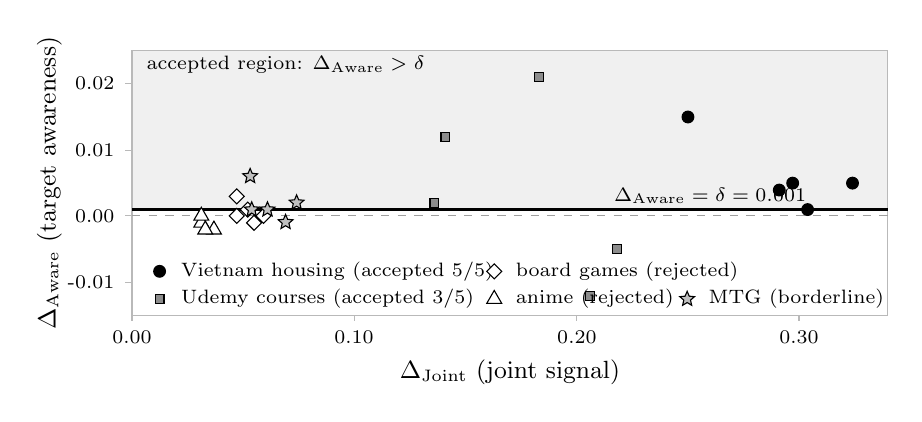
\begin{tikzpicture}[yscale=0.80]

  % acceptance half-plane in Delta_Aware
  \fill[black!6] (0,1.68) rectangle (9.6,4.2);
  % frame
  \draw[gray!55] (0,0) rectangle (9.6,4.2);
  \draw[dashed,gray!75] (0,1.58) -- (9.6,1.58);
  \draw[thick] (0,1.68) -- (9.6,1.68);
  \node[anchor=west,font=\scriptsize] at (0.06,3.98) {accepted region: $\daware > \delta$};
  \node[anchor=west,font=\scriptsize] at (6.0,1.90) {$\daware = \delta = 0.001$};
  % x ticks
  \foreach \x/\l in {0.00/0.00, 2.82/0.10, 5.65/0.20, 8.47/0.30}
    {\draw[gray!55] (\x,0) -- (\x,-0.09); \node[below,font=\scriptsize] at (\x,-0.10) {\l};}
  % y ticks
  \foreach \y/\l in {0.52/-0.01, 1.58/0.00, 2.62/0.01, 3.68/0.02}
    {\draw[gray!55] (0,\y) -- (-0.09,\y); \node[left,font=\scriptsize] at (-0.10,\y) {\l};}
  \node[below,font=\small] at (4.8,-0.55) {$\djoint$ (joint signal)};
  \node[rotate=90,font=\small] at (-1.05,2.1) {$\daware$ (target awareness)};
  % Vietnam
  \node[vmark] at (8.22,1.99) {}; \node[vmark] at (7.06,3.15) {};
  \node[vmark] at (8.39,2.10) {}; \node[vmark] at (8.58,1.68) {};
  \node[vmark] at (9.15,2.10) {};
  % Udemy
  \node[umark] at (5.17,3.78) {}; \node[umark] at (6.16,1.05) {};
  \node[umark] at (5.82,0.31) {}; \node[umark] at (3.84,1.79) {};
  \node[umark] at (3.98,2.83) {};
  % board games
  \node[bmark] at (1.33,1.58) {}; \node[bmark] at (1.33,1.89) {};
  \node[bmark] at (1.47,1.68) {}; \node[bmark] at (1.67,1.58) {};
  \node[bmark] at (1.55,1.47) {};
  % anime
  \node[amark] at (0.88,1.47) {}; \node[amark] at (0.88,1.58) {};
  \node[amark] at (1.04,1.36) {}; \node[amark] at (0.93,1.36) {};
  % MTG card prices: CatBoost, LightGBM, TabM, TabPFN v2, TabPFN-2.5
  \node[mmark] at (1.72,1.68) {}; \node[mmark] at (1.52,1.68) {};
  \node[mmark] at (2.09,1.79) {}; \node[mmark] at (1.50,2.21) {};
  \node[mmark] at (1.95,1.48) {};
  % legend
  \node[vmark] at (0.35,0.70) {}; \node[anchor=west,font=\scriptsize] at (0.5,0.70) {Vietnam housing (accepted 5/5)};
  \node[umark] at (0.35,0.26) {}; \node[anchor=west,font=\scriptsize] at (0.5,0.26) {Udemy courses (accepted 3/5)};
  \node[bmark] at (4.6,0.70) {}; \node[anchor=west,font=\scriptsize] at (4.75,0.70) {board games (rejected)};
  \node[amark] at (4.6,0.26) {}; \node[anchor=west,font=\scriptsize] at (4.75,0.26) {anime (rejected)};
  \node[mmark] at (7.05,0.26) {}; \node[anchor=west,font=\scriptsize] at (7.2,0.26) {MTG (borderline)};
\end{tikzpicture}
\caption{Every gridded (dataset, learner) cell, $\djoint$ against $\daware$, from the per-learner
five-fold means. A learner passes only inside the shaded band.}
\label{fig:scatter}
\end{figure}

\noindent The horizontal spread is much larger than the vertical spread. Joint signal is relatively
easy to find, while target awareness is what eliminates candidates. The three non-accepted
datasets sit far to the left on $\djoint$ and cluster on the acceptance line on $\daware$: of their
fourteen measured learners, only three sit above it, none by more than $+0.006$, while the two
accepted ones clear it on both axes. Nothing in the figure separates accepted from rejected along
the horizontal axis alone.



\section{Vietnam housing - complete T4 grid}
\label{app:vietnam}

\begin{table}[H]
\centering\small
\caption{\textsc{reg\_text\_houses\_vietnam\_2024}, 100 cells (5 learners $\times$ 4 states
$\times$ 5 folds), one Tesla T4, \texttt{ft} at 10 epochs. Sources:
\texttt{grid\_frozen\_gpu.csv}, \texttt{grid\_tar.csv}, \texttt{grid\_tar\_pfn25.csv}.}
\begin{tabular}{lrrrrrrl}
\toprule
Learner & Struct. & Text & Frozen & TAR & $\djoint$ & $\daware$ & Verdict \\
\midrule
CatBoost   & 0.341 & 0.322 & 0.632 & 0.636 & $+0.291$ & $+0.004$ & pass \\
LightGBM   & 0.342 & 0.310 & 0.592 & 0.607 & $+0.250$ & $+0.015$ & pass \\
TabM       & 0.312 & 0.336 & 0.633 & 0.638 & $+0.297$ & $+0.005$ & pass \\
TabPFN v2  & 0.342 & 0.340 & 0.646 & 0.647 & $+0.304$ & $+0.001$ & pass (knife-edge) \\
TabPFN-2.5 & 0.356 & 0.346 & 0.680 & 0.685 & $+0.324$ & $+0.005$ & pass \\
\midrule
\multicolumn{8}{l}{\textbf{5 of 5 pass; quorum 3. ACCEPTED.}} \\
\bottomrule
\end{tabular}
\end{table}

\noindent The grid is complete: zero failed cells and zero soft skips. All five learners pass both terms
against a quorum of three, so the dataset is accepted. The two terms are not comparable in
size. $\djoint$ runs from $+0.250$ to $+0.324$, two orders of magnitude above $\delta$, while
$\daware$ runs from $+0.001$ to $+0.015$ and is the term that could plausibly have failed. TabPFN
v2 passes on a knife edge, its rounded $\daware$ equal to $\delta$; excluding that learner leaves
4 of 5 and the verdict stands.


\begin{table}[H]
\centering\small
\caption{Per-(learner, fold) $\djoint$ (left) and $\daware$ (right), Vietnam housing, unrounded.}
\begin{tabular}{lrrrrr@{\hskip 18pt}rrrrr}
\toprule
& \multicolumn{5}{c}{$\djoint$ by fold} & \multicolumn{5}{c}{$\daware$ by fold} \\
\cmidrule(r){2-6}\cmidrule(l){7-11}
Learner & 0 & 1 & 2 & 3 & 4 & 0 & 1 & 2 & 3 & 4 \\
\midrule
CatBoost   & 0.2847 & 0.2831 & 0.2867 & 0.2924 & 0.2823 & \phantom{-}0.0095 & \phantom{-}0.0110 & 0.0056 & 0.0067 & $-$0.0082 \\
LightGBM   & 0.2424 & 0.2411 & 0.2501 & 0.2661 & 0.2456 & 0.0204 & 0.0188 & 0.0120 & 0.0156 & 0.0110 \\
TabM       & 0.2989 & 0.2958 & 0.2921 & 0.2721 & 0.3137 & 0.0112 & $-$0.0022 & 0.0056 & 0.0043 & 0.0052 \\
TabPFN v2  & 0.2875 & 0.2998 & 0.3039 & 0.2808 & 0.3042 & 0.0063 & 0.0018 & 0.0036 & 0.0019 & $-$0.0064 \\
TabPFN-2.5 & 0.3103 & 0.3292 & 0.3167 & 0.3099 & 0.3097 & 0.0066 & 0.0024 & 0.0071 & 0.0102 & 0.0013 \\
\midrule
\multicolumn{11}{l}{Pooled $\djoint$: $n{=}25$, mean $0.2880$, sd $0.0240$, $25/25$ positive, $t = 59.88$.} \\
\multicolumn{11}{l}{Pooled $\daware$: $n{=}25$, mean $0.0065$, sd $0.0068$, $22/25$ positive, $t = 4.75$, range $[-0.0082, +0.0204]$.} \\
\bottomrule
\end{tabular}
\end{table}

\noindent Pooled over the 25 cells, $\djoint$ is $0.2880 \pm 0.0240$ and positive in every one
($t = 59.88$), while $\daware$ is $0.0065 \pm 0.0068$ and positive in 22 ($t = 4.75$). The three
negative $\daware$ cells fall on three different learners rather than concentrating in one, so no
learner's pass rests on a systematically adverse fold. This is the pattern that distinguishes
this dataset from Udemy courses: the awareness term is small here, but it is consistently
signed.


\clearpage
\section{Udemy courses - complete T4 grid}
\label{app:udemy}

\begin{table}[H]
\centering\small
\caption{\textsc{reg\_text\_edu\_udemy\_academy}, 100 cells, one Tesla T4, \texttt{ft} at 10
epochs. Sources: \texttt{grid\_gpu\_light\_cat\_tabm.csv}, \texttt{grid\_gpu\_tabpfn.csv}.}
\begin{tabular}{lrrrrrrl}
\toprule
Learner & Struct. & Text & Frozen & TAR & $\djoint$ & $\daware$ & Verdict \\
\midrule
CatBoost   & 0.297 & 0.210 & 0.480 & 0.501 & $+0.183$ & $+0.021$ & pass \\
LightGBM   & 0.261 & 0.212 & 0.479 & 0.474 & $+0.218$ & $-0.005$ & fail \\
TabM       & 0.298 & 0.221 & 0.504 & 0.492 & $+0.206$ & $-0.012$ & fail \\
TabPFN v2  & 0.299 & 0.162 & 0.435 & 0.437 & $+0.136$ & $+0.002$ & pass \\
TabPFN-2.5 & 0.311 & 0.211 & 0.452 & 0.464 & $+0.141$ & $+0.012$ & pass \\
\midrule
\multicolumn{8}{l}{\textbf{3 of 5 pass; quorum 3. ACCEPTED.}} \\
\bottomrule
\end{tabular}
\end{table}

\noindent Three of five learners pass, exactly the quorum, so the dataset is accepted. The split falls
entirely on the awareness term: $\djoint$ is large and positive for every learner, from $+0.136$
to $+0.218$, while $\daware$ is negative on LightGBM and on TabM. CatBoost carries the widest
awareness margin at $+0.021$ and TabPFN v2 the narrowest at $+0.002$. An acceptance resting on
the minimum quorum with margins this thin is one we report with the qualification it deserves;
the per-fold table below.


\begin{table}[H]
\centering\small
\caption{Per-(learner, fold) $\djoint$ (left) and $\daware$ (right), Udemy courses, unrounded.}
\begin{tabular}{lrrrrr@{\hskip 18pt}rrrrr}
\toprule
& \multicolumn{5}{c}{$\djoint$ by fold} & \multicolumn{5}{c}{$\daware$ by fold} \\
\cmidrule(r){2-6}\cmidrule(l){7-11}
Learner & 0 & 1 & 2 & 3 & 4 & 0 & 1 & 2 & 3 & 4 \\
\midrule
CatBoost   & 0.1801 & 0.2253 & 0.1411 & 0.2115 & 0.1533 & \phantom{-}0.0029 & \phantom{-}0.0423 & \phantom{-}0.0131 & \phantom{-}0.0069 & \phantom{-}0.0418 \\
LightGBM   & 0.2248 & 0.2431 & 0.1836 & 0.2238 & 0.2054 & $-$0.0169 & $-$0.0005 & 0.0288 & $-$0.0479 & 0.0077 \\
TabM       & 0.2012 & 0.2605 & 0.2252 & 0.1889 & 0.1231 & $-$0.0221 & $-$0.0148 & $-$0.0189 & $-$0.0099 & 0.0067 \\
TabPFN v2  & 0.1318 & 0.1498 & 0.0981 & 0.1429 & 0.1583 & $-$0.0117 & 0.0178 & 0.0068 & 0.0055 & $-$0.0100 \\
TabPFN-2.5 & 0.1301 & 0.1864 & 0.0863 & 0.1433 & 0.1554 & 0.0208 & $-$0.0002 & 0.0133 & 0.0094 & 0.0193 \\
\midrule
\multicolumn{11}{l}{Pooled $\djoint$: $n{=}25$, mean $0.1749$, sd $0.0459$, $25/25$ positive, $t = 19.06$.} \\
\multicolumn{11}{l}{Pooled $\daware$: $n{=}25$, mean $0.0036$, sd $0.0202$, $15/25$ positive, $t = 0.89$ (not significant), range $[-0.0479, +0.0423]$.} \\
\bottomrule
\end{tabular}
\end{table}

\noindent The contrast with Appendix~\ref{app:vietnam} is the point of this table. $\djoint$ is positive in
all 25 cells and pools to $0.1749 \pm 0.0459$ ($t = 19.06$). $\daware$ changes sign within a
single learner across folds - LightGBM spans $-0.0479$ to $+0.0288$ - and pools to
$0.0036 \pm 0.0202$, not significant at $t = 0.89$. A per-learner awareness verdict on this
dataset is therefore a statement about a margin narrower than the fold-to-fold noise, which is
why only the dataset-level verdict should be cited.

\section{Rejected candidates - complete grids}
\label{app:rejected}

\begin{table}[H]
\centering\small
\caption{Board games (\texttt{melissamonfared/board-games}), 100 cells on one T4, measured
with the \emph{maximal} structured block restored.}
\begin{tabular}{lrrrrrrl}
\toprule
Learner & Struct. & Text & Frozen & TAR & $\djoint$ & $\daware$ & Verdict \\
\midrule
CatBoost   & 0.576 & 0.490 & 0.623 & 0.623 & $+0.047$ & $\phantom{-}0.000$ & fail \\
LightGBM   & 0.569 & 0.477 & 0.616 & 0.619 & $+0.047$ & $+0.003$ & pass \\
TabM       & 0.576 & 0.504 & 0.628 & 0.629 & $+0.052$ & $+0.001$ & knife-edge (counted fail) \\
TabPFN v2  & 0.585 & 0.504 & 0.640 & 0.639 & $+0.055$ & $-0.001$ & fail \\
TabPFN-2.5 & 0.586 & 0.514 & 0.645 & 0.645 & $+0.059$ & $\phantom{-}0.000$ & fail \\
\midrule
\multicolumn{8}{l}{\textbf{1 of 5 counted honestly (2 of 5 nominally); quorum 3. REJECTED.}} \\
\multicolumn{8}{l}{Pooled $\djoint$: mean $0.0523$, sd $0.0072$, $25/25$ positive, $t = 36.21$.} \\
\multicolumn{8}{l}{Pooled $\daware$: mean $0.0003$, sd $0.0058$, $10/25$ positive, $t = 0.25$, range $[-0.0124, +0.0163]$.} \\
\bottomrule
\end{tabular}
\end{table}

\noindent $\djoint$ is consistently positive but $\daware$ is not. Every learner clears the joint term, which pools to
$0.0523 \pm 0.0072$ and is positive in all 25 cells, but the awareness term pools to
$0.0003 \pm 0.0058$ with only 10 of 25 cells positive and $t = 0.25$ - indistinguishable
from zero. TabM's $\daware$ of $+0.001$ equals $\delta$ after rounding and is counted as a fail,
which is why the table reads 1 of 5 counted honestly against 2 of 5 nominally. Either count
falls short of the quorum. This candidate is the clearest instance of the pattern in
Figure~\ref{fig:scatter}: a real joint gain that the awareness term nonetheless rejects.


\begin{table}[H]
\centering\small
\caption{Anime popularity (\texttt{wiltheman/anime-data-set-for-ml}, 10{,}000 rows, target
\texttt{popularity}, text $=$ \texttt{genres}, \texttt{themes}, \texttt{title\_english};
\texttt{members} and \texttt{scored\_by} dropped as leakage). 80 cells on one T4.}
\begin{tabular}{lrrrrrrl}
\toprule
Learner & Struct. & Text & Frozen & TAR & $\djoint$ & $\daware$ & Verdict \\
\midrule
CatBoost   & 0.821 & 0.441 & 0.852 & 0.851 & $+0.031$ & $-0.001$ & fail \\
LightGBM   & 0.816 & 0.435 & 0.847 & 0.847 & $+0.031$ & $\phantom{-}0.000$ & fail \\
TabM       & 0.816 & 0.442 & 0.853 & 0.851 & $+0.037$ & $-0.002$ & fail \\
TabPFN v2  & 0.826 & 0.455 & 0.859 & 0.857 & $+0.033$ & $-0.002$ & fail \\
TabPFN-2.5 & \multicolumn{6}{l}{not run} & non-pass \\
\midrule
\multicolumn{8}{l}{\textbf{0 of 5; quorum 3. REJECTED.}} \\
\multicolumn{8}{l}{Pooled $\djoint$: $n{=}20$, mean $0.0329$, sd $0.0066$, $20/20$ positive, $t = 22.31$.} \\
\multicolumn{8}{l}{Pooled $\daware$: $n{=}20$, mean $-0.0012$, sd $0.0026$, $7/20$ positive, $t = -2.15$.} \\
\bottomrule
\end{tabular}
\end{table}

\noindent TabPFN-2.5 was not run, so its cell counts as a non-pass and the quorum denominator stays at
five. The dataset fails at 0 of 5. As with board games the joint term is comfortable, pooling
to $0.0329 \pm 0.0066$ and positive in all 20 measured cells. What sets this candidate apart is
the direction of the awareness term: $\daware$ pools to $-0.0012$ at $t = -2.15$, so the tuned
encoder is significantly \emph{worse} than the frozen one. This is the only candidate we
gridded where adapting the encoder to the target actively hurt.


\begin{table}[H]
\centering\small
\caption{Metacritic PC games - rejected at the target.}
\begin{tabular}{lr}
\toprule
Quantity & Value \\
\midrule
Source rows & 12{,}624 \\
Rows with sentinel \texttt{Metacritic} $= 0$ (``never reviewed'') & 10{,}357 (82\%) \\
Scored rows after repair & 2{,}267 ($20$--$96$, 71 distinct, $|z|_{\max} = 4.67$) \\
Surviving text columns & 1 (\texttt{ResponseName}, a title - a proper noun, not free text) \\
Structured columns & 15, dominated by \texttt{RecommendationCount} (importance $0.62$) \\
Grid completeness & 52 rows, 3 frozen states, no \texttt{ft} state \\
Fold-0 $\daware$ screen & $-0.014$ (LightGBM), $-0.006$ (CatBoost) - wrong sign on both \\
\bottomrule
\end{tabular}
\end{table}

\noindent The rejection happened before a verdict was worth computing. A sentinel \texttt{Metacritic}
score of zero, meaning never reviewed, covers 82\% of rows, so the nominal regression is really
a has-a-score indicator; repairing it leaves 2{,}267 scored rows. The only surviving text
column is a title, a proper noun rather than free text, and the fold-0 $\daware$ screen comes out
the wrong sign on both learners tried. The partial grid is reported for completeness, and no
verdict is claimed from it.


\clearpage
\section{MTG card prices - complete T4 grid, borderline}
\label{app:mtg}

\begin{table}[H]
\centering\small
\caption{\textsc{reg\_text\_games\_mtg\_card\_prices} (\texttt{douglascampospires/mtg-all-cards},
28{,}507 cards, target $\log_{10}(\text{USD})$, text $=$ \texttt{CARD\_TEXT}, \texttt{TYPE}),
100 cells on one T4, \texttt{ft} at 10 epochs. Sources: \texttt{grid\_gpu\_light\_cat\_tabm.csv},
\texttt{grid\_gpu\_tabpfn.csv}.}
\begin{tabular}{lrrrrrrl}
\toprule
Learner & Struct. & Text & Frozen & TAR & $\djoint$ & $\daware$ & Verdict \\
\midrule
CatBoost   & 0.525 & 0.292 & 0.586 & 0.587 & $+0.061$ & $+0.001$ & knife-edge \\
LightGBM   & 0.518 & 0.271 & 0.572 & 0.573 & $+0.054$ & $+0.001$ & knife-edge \\
TabM       & 0.504 & 0.305 & 0.578 & 0.580 & $+0.074$ & $+0.002$ & pass \\
TabPFN v2  & 0.520 & 0.269 & 0.573 & 0.579 & $+0.053$ & $+0.006$ & pass \\
TabPFN-2.5 & 0.523 & 0.310 & 0.592 & 0.591 & $+0.069$ & $-0.001$ & fail \\
\midrule
\multicolumn{8}{l}{\textbf{4 of 5 nominally, 2 of 5 without the knife-edges; quorum 3. BORDERLINE.}} \\
\multicolumn{8}{l}{Pooled $\djoint$: $n{=}25$, mean $0.0620$, sd $0.0108$, $25/25$ positive, $t = 28.85$.} \\
\multicolumn{8}{l}{Pooled $\daware$: $n{=}25$, mean $0.0018$, sd $0.0049$, $18/25$ positive, $t = 1.87$, range $[-0.0122, +0.0096]$.} \\
\bottomrule
\end{tabular}
\end{table}

\noindent The joint term is solid: $\djoint$ is positive in all 25 cells and pools to
$0.0620 \pm 0.0108$ ($t = 28.85$). The awareness term decides the verdict and does not settle
it. The reference implementation passes four learners, but CatBoost and LightGBM clear $\delta$
only on a knife-edge: their rounded $\daware$ equals $\delta$, with unrounded values of
$+0.0009$ and $+0.0011$. Without them, the count is 2 of 5, below quorum. This is the only
candidate whose verdict depends on how knife-edges are counted, so we report it as borderline
and do not count it as an accepted dataset. The target keeps $|z|_{\max} = 5.36$ after the log
transform, which is warned about but never clipped, per the reference protocol.

\section{Validity evidence: the two invalid shortcuts}
\label{app:validity}

\noindent We assessed two plausible ways to cut curation cost, both of which were measurably invalid in that both collapsed the quantity being measured. These were: \textbf{  (1) Deleting structured columns by name.} A filter that drops columns matching \texttt{year} or \texttt{time} removes \texttt{Year
Published} and \texttt{Play Time} from a board-games candidate. These are not identifiers, but two of its strongest structured predictors, so removing them allows the text to proxy for the missing information and creates a joint gain that disappears when the columns are restored. The unstructured baseline never moves, so this is a controlled
ablation rather than a correlation. Name patterns are therefore used only to reject \emph{text}
candidates. \textbf{(2) Cheap screening of $\daware$.} A cheap screening procedure is valid only if reducing computational cost does not alter the quantity being measured. That holds for $\djoint$ (frozen encoders, so a
fold subset is unbiased) and fails for $\daware$ on two independent axes. An under-trained adapter
drives TAR toward frozen by construction, and a single fold cannot resolve a threshold sitting
deep inside the per-(learner, fold) noise band. Screening on one fold cost two full grids.

\begin{table}[H]
\centering\small
\caption{\textbf{Axis 1 - structured-column deletion manufactures $\djoint$.} Board games,
LightGBM, fold 0, target \texttt{Complexity Average}, text $=$ \texttt{Mechanics} $+$
\texttt{Name}.}
\begin{tabular}{lrrrr}
\toprule
Specification & Struct. & Text & Frozen & $\djoint$ \\
\midrule
auto-spec (\texttt{Year Published}, \texttt{Play Time} deleted) & 0.584 & 0.502 & 0.623 & $\mathbf{+0.0388}$ \\
\texttt{Year Published} restored & 0.613 & 0.502 & 0.636 & $+0.0229$ \\
full structured block restored & 0.684 & 0.502 & 0.684 & $\mathbf{-0.0005}$ \\
\midrule
same, semantically natural target (\texttt{Rating Average}) & 0.567 & 0.335 & 0.567 & $+0.0006$ \\
\bottomrule
\end{tabular}
\end{table}

\noindent Columns are restored one at a time. The unstructured baseline never moves from $0.502$, so the
entire effect sits on the structured baseline - which is what makes this a controlled
ablation rather than a correlation. Deleting \texttt{Year Published} and \texttt{Play Time}
yields $\djoint = +0.0388$; restoring \texttt{Year Published} alone cuts that to $+0.0229$;
restoring the full block drives it to $-0.0005$. The apparent joint gain was an artefact of the
deletion at every step, and a semantically natural target behaves the same way at $+0.0006$.
Name patterns are therefore used in this pipeline only to reject \emph{text} candidates, never
to drop structured columns.


\begin{table}[H]
\centering\small
\caption{\textbf{Axis 2a - the epoch budget.} Identical cells, Udemy, fold 0, at two and at
ten epochs.}
\begin{tabular}{lrrrrr}
\toprule
Learner (fold 0) & Frozen & TAR @ 2 ep & $\daware$ @ 2 ep & TAR @ 10 ep & $\daware$ @ 10 ep \\
\midrule
LightGBM & 0.4957 & 0.5056 & $+0.0099$ & 0.5279 & $\mathbf{+0.0322}$ \\
CatBoost & 0.5177 & 0.5282 & $+0.0105$ & 0.5299 & $\mathbf{+0.0122}$ \\
\midrule
\multicolumn{6}{l}{At 2 epochs the full Udemy sweep returned 1 of 5 - an artefact of the budget, not of the dataset.} \\
\bottomrule
\end{tabular}
\end{table}

\noindent An under-trained LoRA adapter leaves TAR close to frozen, collapsing $\daware$ toward zero by
construction. Raising the budget from 2 to 10 epochs more than triples LightGBM's $\daware$, from
$+0.0099$ to $+0.0322$, and moves CatBoost's from $+0.0105$ to $+0.0122$. At 2 epochs the full
Udemy sweep returned 1 of 5 - an artefact of the budget, not a property of the dataset. A
\emph{fail} at a low budget therefore proves nothing. Only a pass is informative. The same
asymmetry is why the 10-epoch budget used throughout can suppress an acceptance but cannot
manufacture one.


\begin{table}[H]
\centering\small
\caption{\textbf{Axis 2b - the fold count.} Fold-0 $\daware$ against the five-fold mean on the
two gridded rejections.}
\begin{tabular}{lrrr@{\hskip 22pt}rrr}
\toprule
& \multicolumn{3}{c}{Board games} & \multicolumn{3}{c}{Anime} \\
\cmidrule(r){2-4}\cmidrule(l){5-7}
Learner & fold 0 & 5-fold & sign & fold 0 & 5-fold & sign \\
\midrule
CatBoost   & $+0.0074$ & $-0.0003$ & \textbf{flip} & $+0.0018$ & $-0.0008$ & \textbf{flip} \\
LightGBM   & $+0.0163$ & $+0.0021$ & --- & $+0.0034$ & $-0.0005$ & \textbf{flip} \\
TabM       & $+0.0052$ & $+0.0010$ & --- & $+0.0010$ & $-0.0016$ & \textbf{flip} \\
TabPFN v2  & $+0.0010$ & $-0.0015$ & \textbf{flip} & $-0.0041$ & $-0.0020$ & --- \\
TabPFN-2.5 & $+0.0064$ & $+0.0001$ & --- & \multicolumn{3}{c}{not run} \\
\midrule
\multicolumn{7}{l}{Per-(learner, fold) spread: board games $\sigma = 0.0058$ over $[-0.0124, +0.0163]$; anime $\sigma = 0.0026$} \\
\multicolumn{7}{l}{over $[-0.0066, +0.0034]$. The threshold $\delta = 0.001$ sits inside both bands, so one fold cannot} \\
\multicolumn{7}{l}{resolve the criterion. Screening on one fold cost two full grids.} \\
\bottomrule
\end{tabular}
\end{table}

\noindent Every board-games learner drops between the two columns and two change sign. Anime's positive
fold-0 reading reverses entirely, with three of its four measured learners flipping. The
per-(learner, fold) spread quoted at the foot of the table puts $\delta = 0.001$ well inside
both noise bands, so a single fold cannot resolve the criterion in either direction. We
screened on one fold before establishing this, and it cost two full grids.


\clearpage
\section{Screen-time rejections}
\label{app:screen}

\begin{table}[H]
\centering\small
\caption{Candidates rejected before a full grid was spent, each with the measured quantity
that condemns it.}
\begin{tabular}{p{0.30\textwidth}p{0.60\textwidth}}
\toprule
Candidate & Reason (with the measured quantity that condemns it) \\
\midrule
\texttt{steam-games-dataset-steamspy} & auto-target was \texttt{appid}, a primary key; no free text besides proper nouns \\
\texttt{gog-com-video-games} & auto-target was a date; re-screened $\djoint = -0.0003$, text $R^2 = 0.996$ (the text \emph{was} the release dates) \\
\texttt{popular-video-games-1980-2023} & 1{,}512 rows; no numeric column qualified as a target \\
\texttt{lego-sets} & 12{,}261 rows are 744 products replicated across 21 countries --- near-duplicates straddle train and test \\
\texttt{top-women-chess-players} & $\djoint = +0.024$ inside the $\pm 0.015$ band, text $R^2 = 0.074$ (text nearly inert) \\
\texttt{kerala-bevco-liquor-price} & auto-target was \texttt{Sl No}; with the corrected target, structured $R^2 = 1.000$ (deterministic) \\
\texttt{google-play-store-apps} & target derived from its own text \\
\texttt{daraz-perfumes} & every state negative ($-0.130$ / $-0.009$ / $-0.045$): a delta between them is meaningless \\
\texttt{global-grocery-nutrition-2025} & $\djoint = +0.0005$ with structured $R^2 = 0.969$ --- saturated, no headroom \\
\texttt{global-movies-1950-2026} & target \texttt{roi\_pct} $=$ revenue/budget, an arithmetic identity over two structured columns; structured $R^2 = 0.997$ \\
\texttt{steam-games-dataset} & no numeric column qualified as a target \\
\texttt{ultimate-games-15k} & auto-target was \texttt{serial\_no}; $\djoint = -0.0027$ against structured $R^2 = 0.983$ \\
\texttt{horror-movies-profits} & $\djoint$ healthy ($+0.055$ / $+0.093$) but fold-0 $\daware$ $-0.001$ / $-0.013$ \\
\texttt{vgsales-userscore} & every delta at noise scale: $\djoint$ $+0.001$/$+0.004$, $\daware$ $+0.001$/$+0.002$ \\
\bottomrule
\end{tabular}
\end{table}

\noindent Two classes recur. The first is a junk target chosen automatically: \texttt{appid},
\texttt{Sl No} and \texttt{serial\_no} are primary keys or serial numbers, and one candidate
had a release date selected as its target. The second is a saturated or degenerate baseline
against which no text signal can be demonstrated, with structured $R^2$ reaching $0.969$,
$0.983$, $0.997$ and $1.000$ on four separate candidates. Both classes are cheap to detect from
a profile of the target and the structured block, and neither needs a grid to rule out - which
is what makes the profiling stage of the funnel worth its cost.


\section{Harness validation against the benchmark's own anchor}
\label{app:anchor}

\begin{table}[H]
\centering\small
\caption{Anchor dataset \textsc{mul\_text\_product\_sentiment} ($N = 5{,}091$, 4 classes,
1 text $+$ 1 structured column); 36-run frozen grid.}
\begin{tabular}{lr}
\toprule
Check & Result \\
\midrule
Published $56 \times 10$ pass matrix re-derived from released scores & \textbf{0 mismatched cells} \\
Verdict function on a known accepted dataset & accepted, 5 of 5 \\
Verdict function on a known rejected dataset & rejected, 0 of 5 \\
\texttt{no\_text} (encoder-free) vs published, mean absolute difference & \textbf{0.0000} \\
\quad LightGBM \texttt{no\_text}, fold 0 & $0.83454303717305$ (identical) \\
\texttt{text\_only} vs published, mean signed difference & $-0.0000$ (range $-0.046$ to $+0.038$) \\
\texttt{all} vs published, mean signed difference & $+0.0058$ (max $+0.0235$) \\
Frozen-embedding cache, cached vs uncached score & $0.8618478948517495$, bit-identical \\
\bottomrule
\end{tabular}
\end{table}

\noindent These checks ran before any candidate number was trusted. The published $56 \times 10$ pass
matrix re-derives from the released scores with zero mismatched cells, and the verdict function
returns the published outcome on both a known accepted and a known rejected dataset. The
encoder-free \texttt{no\_text} condition reproduces published scores exactly - to fourteen
decimal places on the LightGBM fold-0 cell - which pins loading, curation, splitting and
seeding. The encoder-dependent conditions agree less tightly, \texttt{all} carrying a
$+0.0058$ mean signed difference. That gap is the expected consequence of a different embedding
environment, not of a different protocol, and it is why the next table validates $\djoint$ itself
rather than the raw scores it is built from.


\begin{table}[H]
\centering\small
\caption{$\djoint$ - the quantity the criterion consumes - reproduced on the anchor.}
\begin{tabular}{lrrr}
\toprule
Learner & $\djoint$ (ours) & $\djoint$ (published) & Sign agrees \\
\midrule
CatBoost  & 0.075 & 0.073 & yes \\
LightGBM  & 0.058 & 0.046 & yes \\
TabM      & 0.085 & 0.086 & yes \\
TabPFN v2 & 0.076 & 0.079 & yes \\
\bottomrule
\end{tabular}
\end{table}

\noindent The deltas agree within $0.012$ across four learners with every sign agreeing, and three of the
four agree within $0.003$. The single wider case is LightGBM, at $0.058$ against a published
$0.046$. This reproduction is the calibration behind the $\pm 0.015$ fold-noise band used
throughout the paper: a candidate whose $\djoint$ falls inside that band is not distinguishable
from measurement noise, and is screened out rather than gridded.



\end{document}